\section*{Seminár 1}

\section*{Seminár 2}

\section*{Seminár 3}

\noindent \ul{3.1}  Pre ľubovoľné reálne čísla $x, y$ a $z$ dokážte nezápornosť hodnoty každého z~výrazov $$x^2z^2+ y^2- 2xyz, \ x^2+ 4y^2+ 3z^2- 2x - 12y - 6z + 13, \ 2x^2+ 4y^2 + z^2- 4xy - 2xz$$ a zistite tiež, kedy je dotyčná hodnota rovná nule.



\noindent \ul{3.2} 
a)Určte najmenšiu hodnotu výrazu $V = 5 + (x - 2)^2$, $x \in \RR$. Pre ktoré $x$ ju výraz nadobúda?

b) Určte najmenšiu možnú hodnotu výrazu $W = 9 - ab$, kde $a, b$ sú reálne čísla spĺňajúce podmienku $a + b = 6$. Pre ktoré hodnoty $a, b$ je $W$ minimálne?

c) Určte najmenšiu možnú hodnotu výrazu $Y = 12-ab$, kde $a, b$ sú reálne čísla spĺňajúce podmienku $a + b = 6$. Pre ktoré hodnoty $a, b$ je $Y$ minimálne?

d) Určte najväčšiu možnú hodnotu výrazu $K = 5 + ab$, kde $a, b$ sú reálne čísla spĺňajúce podmienku $a + b = 8$. Pre ktoré hodnoty $a, b$ je $K$ maximálne?




\noindent \ul{3.3}  Určte, akú najmenšiu hodnotu môže nadobúdať výraz $V = (a-b)^2 +(b-c)^2 +(c-a)^2$, ak reálne čísla $a, b, c$ spĺňajú dvojicu podmienok
\begin{align*}
a + 3b + c &= 6,\\
-a + b - c &= 2.
\end{align*}




\noindent \ul{3.4}  Určte, aké hodnoty môže nadobúdať výraz $V = ab + bc + cd + da$, ak reálne čísla $a,b, c, d$ spĺňajú dvojicu podmienok
\begin{align*}
2a - 5b + 2c - 5d &= 4,\\
3a + 4b + 3c + 4d &= 6.
\end{align*}



\noindent \ul{3.5}  Uvažujme výraz $$2x^2+ y^2 - 2xy + 2x + 4.$$
\begin{enumerate}[a)]

\item Nájdite všetky reálne čísla $x$ a $y$, pre ktoré daný výraz nadobúda svoju najmenšiu hodnotu.

\item Určte všetky dvojice celých nezáporných čísel $x$ a $y$, pre ktoré je hodnota daného výrazu rovná číslu 16.
\end{enumerate}



\noindent \ul{3.6}  Nájdite najmenšiu možnú hodnotu výrazu $$3x^2 - 12xy + y^4,$$
v~ktorom $x$ a $y$ sú ľubovoľné celé nezáporné čísla.




\noindent \ul{3.7}  V~obore celých čísel vyriešte rovnicu $x^2+ y^2+ x + y = 4$.




\section*{Seminár 4}

\noindent \ul{4.1} 
Dokážte, že pre ľubovoľné nezáporné čísla $a, b, c$ platí $$(a + bc)(b + ac) \geq ab(c + 1)^2.$$
Zistite, kedy nastane rovnosť.




\noindent \ul{4.2}  Dokážte, že pre ľubovoľné reálne čísla $x$, $y$ a $z$ platia nerovnosti
\begin{enumerate}[a)]
\item $2xyz \leq x^2+ y^2z^2$,
\item $(x^2-y^2)^2\geq 4xy(x - y)^2$.
\end{enumerate}





\noindent \ul{4.3}  Dokážte, že pre ľubovoľné kladné čísla $a$, $b$ platí nerovnosť $$\frac{a}{b^2}+ \frac{b}{a^2}\geq \frac{1}{a} + \frac{1}{b}.$$




\noindent \ul{4.4}  Dokážte nerovnosť $$\frac{1}{ab}+\frac{1}{cd}\geq \frac{8}{(a+b)(c+d)},$$ pre ľubovoľné kladné čísla $a, b, c, d$.




\noindent \ul{4.5}  Dokážte, že pre ľubovoľné reálne číslo a platí nerovnosť $$a^2+\frac{1}{a^2-a+1}\geq a+1.$$ Určte, kedy nastáva rovnosť.




\noindent \ul{4.6}  Dokážte, že pre ľubovoľné kladné reálne čísla $a, b$ platí
$$ \sqrt{ab}\leq \frac{2(a^2+3ab+b^2)}{5(a+b)}\leq \frac{a+b}{2},$$
a pre každú z~oboch nerovností zistite, kedy prechádza na rovnosť.




\noindent \ul{4.7} 
Dokážte, že pre ľubovoľné kladné čísla $a, b, c$ platí nerovnosť
$$\bigg(a +\frac{1}{b}\bigg)\bigg(b+\frac{1}{c}\bigg)\bigg(c+\frac{1}{a}\bigg)\geq 8$$
a zistite, kedy prechádza v~rovnosť.




\noindent \ul{4.8} 
Dokážte, že pre ľubovoľné čísla $a, b$ z~intervalu $\langle 1, \infty)$ platí nerovnosť
$$ (a^2 + 1)(b^2 + 1) - (a - 1)^2 (b - 1)^2 \geq 4$$
a zistite, kedy nastane rovnosť.




\noindent \ul{4.9} 
Dokážte, že pre ľubovoľné rôzne kladné čísla $a, b$ platí
$$\frac{a+b}{2}<\frac{2(a^2 + ab + b^2 )}{3(a+b)}<\sqrt{\frac{a^2+b^2}{2}}.$$




\section*{Seminár 5}

\noindent \ul{5.1}  Máme tri čísla so súčtom 2010, pričom každé z~nich je aritmetickým priemerom zvyšných dvoch. Aké sú to čísla?




\noindent \ul{5.2}  Máme tri čísla, o~ktorých vieme, že každé z~nich je aritmetickým priemerom niektorých dvoch z~našich troch čísel. Dokážte, že naše tri čísla sú rovnaké.




\noindent \ul{5.3} 
Lucia napísala na tabuľu dve nenulové čísla. Potom medzi ne postupne vkladala znamienka plus, mínus, krát a delené a všetky štyri príklady správne vypočítala. Medzi výsledkami boli iba dve rôzne hodnoty. Aké dve čísla mohla Lucia na tabuľu napísať?




\noindent \ul{5.4} 
Na tabuli sú napísané práve tri (nie nutne rôzne) reálne čísla. Vieme, že súčet ľubovoľných dvoch z~nich je tam napísaný tiež. Určte všetky trojice takých čísel.




\noindent \ul{5.5} 
Po okruhu behajú dvaja atléti, každý inou konštantnou rýchlosťou. Keď bežia opačnými smermi, stretávajú sa každých 10 minút, keď bežia rovnakým smerom, stretávajú sa každých 40 minút. Za aký čas zabehne okruh rýchlejší atlét?




\noindent \ul{5.6}  Určte všetky dvojčleny $P (x) = ax + b$, pre ktoré platí $P(2) = 3$ a $P (3) = 2$.




\noindent \ul{5.7}  Určte všetky trojčleny $P (x) = ax^2+ bx + c$, pre ktoré platí $P (1) = 4$, $P (2) = 9$ a $P (3) = 18$.




\noindent \ul{5.8}  Určte všetky dvojčleny $P (x) = ax+b$ s~celočíselnými koeficientmi $a$ a $b$, pre ktoré platí $P (1) < P (2)$ a $P (1)^2+ P(2)^2= 5$.




\noindent \ul{5.9}  Koeficienty $a, b, c$ trojčlena $P (x) = ax^2+ bx + c$ sú reálne čísla, pritom každá z~troch jeho hodnôt $P (1), P (2)$ a $P (3)$ je celým číslom. Vyplýva z~toho, že aj čísla $a, b, c$ sú celé, alebo je nutne celé aspoň niektoré z~nich (ktoré)?




\noindent \ul{5.10}  Nájdite všetky dvojice nezáporných celých čísel $a$, $b$, pre ktoré platí
$$a^2 + b + 2 = a + b^2.$$




\noindent \ul{5.11} 
Nájdite všetky trojčleny $P(x)=ax^2+bx+c$ s~celočíselnými koeficientami $a, b, c$, pre ktoré platí $P(1) < P(2) < P(3)$ a zároveň $$(P(1))^2+ (P(2))^2+ (P(3))^2= 22.$$



\noindent \ul{5.12} 
Nájdite všetky dvojice celých kladných čísel $a$ a $b$, pre ktoré je číslo $a^2 +b$ o~62 väčšie
ako číslo $b^2 + a$.




\noindent \ul{5.13}  Nech $n$ je prirodzené číslo väčšie ako 2. Máme $n$ čísel so súčtom $n$, pričom každé z~nich je aritmetickým priemerom ostatných čísel. Aké sú to čísla?




\section*{Seminár 6}

\noindent \ul{6.1}  Nech $N$ je päťciferné kladné číslo také, že $N=\overline{a679b}$. Ak je $N$ deliteľné 72, určte prvú cifru $a$ a poslednú cifru $b$.




\noindent \ul{6.2}  Dokážte, že v~nekonečnom rade čísel
$$ 1 \cdot 2 \cdot 3, 2 \cdot 3 \cdot 4, 3 \cdot 4 \cdot 5, 4 \cdot 5 \cdot 6, \ldots ,$$
je číslo prvé deliteľom všetkých čísel ďalších.




\noindent \ul{6.3}  Dokážte, že pre každé prirodzené $n$ je číslo $n^3+ 2n$ deliteľné tromi.




\noindent \ul{6.4}  Dokážte, že pre každé nepárne číslo $n$ je číslo $n^2 - 1$ deliteľné ôsmimi.




\noindent \ul{6.5}  \begin{enumerate}[a)]
\item Dokážte, že pre všetky celé kladné čísla $m$ je rozdiel $m^6 - m^2$ deliteľný šesťdesiatimi.
\item Určte všetky kladné celé čísla $m$, pre ktoré je rozdiel $m^6 - m^2$ deliteľný číslom 120.
\end{enumerate}



\noindent \ul{6.6} 
Dokážte, že pre ľubovoľné celé čísla $n$ a $k$ väčšie ako 1 je číslo $n^{k+2} - n^k$ deliteľné dvanástimi.




\noindent \ul{6.7} 
Keď isté dve prirodzené čísla v~rovnakom poradí sčítame, odčítame, vydelíme a vynásobíme a všetky štyri výsledky sčítame, dostaneme 2 009. Určte tieto dve čísla.




\noindent \ul{6.8}  Nájdite všetky celé $d > 1$, pri ktorých hodnoty výrazov $U(n) = n^3+ 17n^2-1$ a $V (n) = n^3+ 4n^2+ 12$ dávajú po delení číslom $d$ rovnaké zvyšky, nech je celé číslo $n$ zvolené akokoľvek.




\noindent \ul{6.9}  Pre ktoré prirodzené čísla $n$ nie je výraz $V (n) = n^4+ 11n^2 - 12$ násobkom ôsmich?




\noindent \ul{6.10} 
Nájdite najväčšie prirodzené číslo $d$, ktoré má tú vlastnosť, že pre ľubovoľné prirodzené číslo $n$ je hodnota výrazu $$V (n) = n^4+ 11n^2-12$$
deliteľná číslom $d$.




\noindent \ul{6.11} 
Označme $M$ množinu všetkých hodnôt výrazu $V (n) = n^4 + 11n^2 - 12$, pričom $n$ je nepárne prirodzené číslo. Nájdite všetky možné zvyšky po delení číslom 48, ktoré dávajú prvky množiny $M$.




\noindent \ul{6.12} 
Dokážte, že výrazy $23x + y$, $19x + 3y$ sú deliteľné číslom 50 pre rovnaké dvojice prirodzených čísel $x$, $y$.




\section*{Seminár 7}

\noindent \ul{7.1}  Určte, pre ktoré prirodzené čísla $a, b$ platí $(a, b) = 10$ a zároveň  $[a, b] = 150$.




\noindent \ul{7.2}  Nech $d$ je najväčší spoločný deliteľ prirodzených čísel $a$ a $b$. Ukážte, že čísla $a/d$ a $b/d$ sú celé a nesúdeliteľné.




\noindent \ul{7.3}  Dokážte, že pre ľubovoľné prirodzené čísla $a, b$ platí vzťah $$[a, b] \cdot (a, b) = ab.$$




\noindent \ul{7.4}  Platí pre každé tri prirodzené čísla $a, b, c$ a ich najväčší spoločný deliteľ $d$ a ich najmenší spoločný násobok $n$ rovnosť $abc = nd$?




\noindent \ul{7.5}  Ak majú prirodzené čísla $a, b$ najväčšieho spoločného deliteľa $d$, majú rovnakého najväčšieho spoločného deliteľa aj čísla $a$, $b$, $a - b$, $a + b$. Dokážte. Platí rovnaké tvrdenie pre najmenší spoločný násobok?




\noindent \ul{7.6}  Nájdite všetky dvojice prirodzených čísel $a, b$, pre ktoré platí $a+b+[a, b]+(a, b) = 50$.




\noindent \ul{7.7} 
Nájdite všetky dvojice prirodzených čísel $a, b$, pre ktoré platí rovnosť množín
$$\{a \cdot [a, b], b \cdot (a, b)\} = \{45, 180\}.$$




\noindent \ul{7.8} 
Rozdiel dvoch prirodzených čísel je $2010$ a ich najväčší spoločný deliteľ je $2014$-krát menší ako ich najmenší spoločný násobok. Určte všetky také dvojice čísel.




\noindent \ul{7.9}  Nájdite všetky dvojice kladných celých čísel $a, b$, pre ktoré má výraz
$$\frac{a}{b}+\frac{14b}{9a}$$
celočíselnú hodnotu.




\noindent \ul{7.10} 
Dokážte, že najmenší spoločný násobok $[a, b]$ a najväčší spoločný deliteľ $(a, b)$ ľubovoľných dvoch kladných celých čísel $a, b$ spĺňajú nerovnosť
$$a \cdot (a, b) + b \cdot [a, b] \geq 2ab.$$
Zistite, kedy v~tejto nerovnosti nastane rovnosť.




\noindent \ul{7.11} 
Nájdite všetky trojice prirodzených čísel $a, b, c$, pre ktoré platí množinová rovnosť
$$\{(a, b), (a, c), (b, c), [a, b], [a, c], [b, c]\}= \{2, 3, 5, 60, 90, 180\},$$
pričom $(x, y)$ a $[x, y]$ označuje postupne najväčší spoločný deliteľ a najmenší spoločný násobok čísel $x$ a $y$.




\noindent \ul{7.12} 
Čísla 1, 2, \ldots , 10 rozdeľte na dve skupiny tak, aby najmenší spoločný násobok súčinu všetkých čísel prvej skupiny a súčinu všetkých čísel druhej skupiny bol čo najmenší.




\section*{Seminár 8}

\noindent \ul{8.1}  Trojciferné číslo sa končí cifrou 4. Ak túto cifru presunieme na prvé miesto (a ostatné dve cifry necháme bez zmeny), dostaneme číslo, ktoré je o~81 menšie ako pôvodné číslo. Určte pôvodné číslo.




\noindent \ul{8.2}  Nájdite všetky prirodzené dvojciferné čísla, ktoré sa rovnajú dvojnásobku súčinu svojich cifier.




\noindent \ul{8.4}  Janko má tri kartičky, na každej je iná nenulová cifra. Súčet všetkých trojciferných čísel, ktoré možno z~týchto kartičiek zostaviť, je číslo o~6 väčšie ako trojnásobok jedného z~nich. Aké cifry sú na kartičkách?




\noindent \ul{8.5} 
Nájdite všetky trojice (nie nutne rôznych) cifier $a, b, c$ také, že päťciferné čísla $\overline{6abc3}$ a $\overline{3abc6}$ sú v~pomere 63 : 36.




\noindent \ul{8.6}   Žiaci mali vypočítať príklad $x + y \cdot z$ pre trojciferné číslo $x$ a dvojciferné čísla $y, z$. Martin vie násobiť a sčítať čísla zapísané v~desiatkovej sústave, ale zabudol na pravidlo prednosti násobenia pred sčítaním. Preto mu vyšlo síce zaujímavé číslo, ktoré sa píše rovnako zľava doprava ako sprava doľava, správny výsledok bol ale o~$2 004$ menší. Určte čísla $x, y, z$.




\noindent \ul{8.7}  Určte počet všetkých štvorciferných prirodzených čísel, ktoré sú deliteľné šiestimi a v~ktorých zápise sa vyskytujú práve dve jednotky.




\noindent \ul{8.8}   Určte počet všetkých trojíc dvojciferných prirodzených čísel $a$, $b$, $c$, ktorých súčin $abc$ má zápis, v~ktorom sú všetky cifry rovnaké. Trojice líšiace sa len poradím čísel považujeme za rovnaké,  t.\,j. započítavame ich iba raz.




\noindent \ul{8.9}  Nájdite všetky štvorciferné čísla $n$, ktoré majú nasledujúce tri vlastnosti: V~zápise čísla $n$ sú dve rôzne cifry, každá dvakrát. Číslo $n$ je deliteľné siedmimi. Číslo, ktoré vznikne otočením poradia cifier čísla $n$, je tiež štvorciferné a deliteľné siedmimi.




\noindent \ul{8.10}  Klárka mala na papieri napísané trojciferné číslo. Keď ho správne vynásobila deviatimi, dostala štvorciferné číslo, ktoré sa začínalo rovnakou číslicou ako pôvodné číslo, prostredné dve číslice sa rovnali a posledná číslica bola súčtom číslic pôvodného čísla. Ktoré štvorciferné číslo mohla Klárka dostať?




\section*{Seminár 9}

\noindent \ul{9.1} Dokážte, že súčet veľkostí vnútorných uhlov ľubovoľného trojuholníka je $180^\circ$.\ul{9.1} Dokážte, že súčet veľkostí vnútorných uhlov ľubovoľného trojuholníka je $180^\circ$.




\noindent \ul{9.2}  Z~trojuholníkových nerovností medzi dĺžkami strán ľubovoľného trojuholníka odvoďte známe
pravidlo $\alpha < \beta \Rightarrow a < b$ o~porovnaní veľkostí vnútorných uhlov a dĺžok protiľahlých strán v~ľubovoľnom trojuholníku $ABC$.




\noindent \ul{9.3}  Dokážte vety:

a) Ak majú dva trojuholníky rovnakú výšku, potom pomer ich obsahov sa rovná pomeru dĺžok príslušných základní.

b) Ak majú dva trojuholníky zhodné základne, potom pomer ich obsahov sa rovná pomeru príslušných výšok.




\noindent \ul{9.4}   Pre všeobecný trojuholník $ABC$ so stranami $a$, $b$, $c$ a obsahom $S$ platí pre polomer $r$ vpísanej kružnice vzorec $r = 2S/(a + b + c)$. Dokážte.




\noindent \ul{9.5} Dokážte, že uhlopriečky v~rovnobežníku sa navzájom polia.\ul{9.5} Dokážte, že uhlopriečky v~rovnobežníku sa navzájom polia.




\noindent \ul{9.6}   Označme $U$ priesečník uhlopriečok daného konvexného štvoruholníka $ABCD$. Dokážte, že priamky $AB$ a $CD$ sú rovnobežné práve vtedy, keď trojuholníky $ADU$ a $BCU$ majú rovnaký obsah.




\noindent \ul{9.7}  Lichobežník $ABCD$ má základne s~dĺžkami $|AB|=a$ a $|CD|=C$ a jeho uhlopriečky sa pretínajú v~bode $U$. Aký je pomer obsahov trojuholníkov $ABU$ a $CDU$?




\noindent \ul{9.8}  Nech $k$ je kružnica opísaná pravouhlému trojuholníku $ABC$ s~preponou $AB$ dĺžky $c$. Označme $S$ stred strany $AB$ a $D$ a $E$ priesečníky osí strán $BC$ a $AC$ s~jedným oblúkom $AB$ kružnice $k$. Vyjadrite obsah trojuholníka $DSE$ pomocou dĺžky prepony $c$.




\noindent \ul{9.9}  Vyjadrite obsah rovnoramenného lichobežníka $ABCD$ so základňami $AB$ a $CD$ pomocou dĺžok $a$, $c$ jeho základní a dĺžky $b$ jeho ramien.




\noindent \ul{9.10} Použitím viet o~podobnosti trojuholníkov a Pytagorovej vety odvoďte Euklidove vety o~odvesne a o~výške pravouhlého trojuholníka.\ul{9.10} Použitím viet o~podobnosti trojuholníkov a Pytagorovej vety odvoďte Euklidove vety o~odvesne a o~výške pravouhlého trojuholníka.



\section*{Seminár 10}

\noindent \ul{10.1}  Päta $P$ výšky z~vrcholu $C$ v~trojuholníku $ABC$ delí stranu $AB$ v~pomere $|AP| : |PB|= 1 : 3$. V~rovnakom pomere sú aj obsahy štvorcov nad jeho stranami $AC$ a $BC$.
Dokážte, že trojuholník $ABC$ je pravouhlý.



\noindent \ul{10.2} 
Päta výšky z~vrcholu $C$ v~trojuholníku $ABC$ delí stranu $AB$ v~pomere $1 : 2$. Dokážte, že pri zvyčajnom označení dĺžok strán trojuholníka $ABC$ platí nerovnosť $$3|a - b| < c.$$



\noindent \ul{10.3} 
Daný je trojuholník $ABC$ s~pravým uhlom pri vrchole $C$. Stredom $I$ kružnice trojuholníku vpísanej vedieme rovnobežky so stranami $CA$ a $CB$, ktoré pretnú preponu postupne v~bodoch $X$ a $Y$. Dokážte, že platí $|AX|^2 + |BY |^2 = |XY |^2$.




\noindent \ul{10.4} 
 V~pravouhlom trojuholníku $ABC$ označíme $P$ pätu výšky z~vrcholu $C$ na preponu $AB$. Priesečník úsečky $AB$ s~priamkou, ktorá prechádza vrcholom $C$ a stredom kružnice vpísanej trojuholníku $PBC$, označíme $D$. Dokážte, že úsečky $AD$ a $AC$ sú zhodné.




\noindent \ul{10.5}  Označme $E$ stred základne $AB$ lichobežníka $ABCD$, v~ktorom platí $|AB| : |CD| = 3 : 1$. Uhlopriečka $AC$ pretína úsečky $ED$, $BD$ postupne v~bodoch $F$, $G$. Určte postupný pomer $|AF| : |FG| : |GC|$.




\noindent \ul{10.6}  Vo štvorci $ABCD$ označme $K$ stred strany $AB$ a $L$ stred strany $AD$. Úsečky $KD$ a $LC$ sa pretínajú v~bode $M$ a rozdeľujú štvorec na dva trojuholníky a dva štvoruholníky. Vypočítajte ich obsahy, ak úsečka $LM$ má dĺžku 1\,cm.




\noindent \ul{10.7}  V~pravouhlom lichobežníku $ABCD$ s~pravým uhlom pri vrchole $A$ základne $AB$ je bod $K$ priesečníkom výšky $CP$ lichobežníka s~jeho uhlopriečkou $BD$. Obsah štvoruholníka $APCD$ je polovicou obsahu lichobežníka $ABCD$. Určte, akú časť obsahu trojuholníka $ABC$ zaberá trojuholník $BCK$.




\noindent \ul{10.8}  Pravouhlému trojuholníku $ABC$ s~preponou $AB$ je opísaná kružnica. Päty kolmíc z~bodov $A$, $B$ na dotyčnicu k~tejto kružnici v~bode $C$ označme $D$, $E$. Vyjadrite dĺžku úsečky $DE$ pomocou dĺžok odvesien trojuholníka $ABC$.




\noindent \ul{10.9} 
V~pravouhlom trojuholníku $ABC$ označíme $P$ pätu výšky z~vrcholu $C$ na preponu $AB$ a $D, E$ stredy kružníc vpísaných postupne trojuholníkom $APC$, $CPB$. Dokážte, že stred
kružnice vpísanej trojuholníku $ABC$ je priesečníkom výšok trojuholníka $CDE$.




\section*{Seminár 11}

\noindent \ul{11.1}  V~danom rovnobežníku $ABCD$ je bod $E$ stred strany $BC$ a bod $F$ leží vnútri strany $AB$. Obsah trojuholníka $AFD$ je $15$\,cm$^2$ a obsah trojuholníka $FBE$ je $14$\,cm$^2$. Určte obsah štvoruholníka $FECD$.




\noindent \ul{11.2}  Vnútri rovnobežníka $ABCD$ je daný bod $K$ a v~páse medzi rovnobežkami $BC$ a $AD$ v~polrovine opačnej k~$CDA$ je daný bod $L$. Obsahy trojuholníkov $ABK, BCK, DAK$ a $DCL$ sú $S_{ABK} = 18$\,cm$^2$, $S_{BCK} = 8$\,cm$^2$, $S_{DAK} = 16$\,cm$^2$, $S_{DCL} = 36$\,cm$^2$. Vypočítajte obsahy trojuholníkov $CDK$ a $ABL$.




\noindent \ul{11.3}  Označme $K$ a $L$ postupne body strán $BC$ a $AC$ trojuholníka $ABC$, pre ktoré platí $|BK|= \frac{1}{3}|BC|$, $|AL| =\frac{1}{3}|AC|$. Nech $M$ je priesečník úsečiek $AK$ a $BL$. Vypočítajte pomer obsahov trojuholníkov $ABM$ a $ABC$.




\noindent \ul{11.4}   Daný je lichobežník $ABCD$ so základňami $AB$, $CD$, pričom $2|AB| = 3|CD|$.

a) Nájdite bod $P$ vnútri lichobežníka tak, aby obsahy trojuholníkov $ABP$ a $CDP$ boli v~pomere $3 : 1$ a aj obsahy trojuholníkov $BCP$ a $DAP$ boli v~pomere $3 : 1$.

b) Pre nájdený bod $P$ určte postupný pomer obsahov trojuholníkov $ABP$, $BCP$, $CDP$ a $DAP$.




\noindent \ul{11.5}  Vnútri pravidelného šesťuholníka $ABCDEF$ s~obsahom 30\,cm$^2$ je zvolený bod $M$. Obsahy trojuholníkov $ABM$ a $BCM$ sú postupne 3\,cm$^2$ a 2\,cm$^2$. Určte obsahy trojuholníkov $CDM$, $DEM$, $EFM$ a $FAM$.




\noindent \ul{11.6}  Vnútri strán $AB$, $AC$ daného trojuholníka $ABC$ sú zvolené postupne body $E$, $F$, pričom $EF \parallel BC$. Úsečka $EF$ je potom rozdelená bodom $D$ tak, že platí $$p = |ED| : |DF | = |BE| : |EA|.$$

a) Ukážte, že pomer obsahov trojuholníkov $ABC$ a $ABD$ je pre $p = 2 : 3$ rovnaký ako pre $p = 3 : 2$.

b) Zdôvodnite, prečo pomer obsahov trojuholníkov $ABC$ a $ABD$ má hodnotu aspoň 4.




\section*{Seminár 12}

\noindent \ul{12.1}  Trojuholník $ABC$ spĺňa pri zvyčajnom označení dĺžok strán podmienku $a \leq b \leq c$. Vpísaná kružnica sa dotýka strán $AB$, $BC$ a $AC$ postupne v~bodoch $K$, $L$ a $M$. Dokážte, že z~úsečiek $AK$, $BL$ a $CM$ možno zostrojiť trojuholník práve vtedy, keď platí $b + c < 3a$.




\noindent \ul{12.2}  Označme $S$ stred základne $AB$ daného rovnoramenného trojuholníka $ABC$. Predpokladajme, že kružnice vpísané trojuholníkom $ACS$, $BCS$ sa dotýkajú priamky $AB$ v~bodoch, ktoré delia základňu $AB$ na tri zhodné diely. Vypočítajte pomer $|AB| : |CS|$.




\noindent \ul{12.3}  Danému rovnostrannému trojuholníku vpíšme a opíšme kružnicu. Označme $S$ obsah vzniknutého medzikružia a $T$ obsah kruhu, ktorého priemer je zhodný s~dĺžkou strany daného trojuholníka. Ktorý z~obsahov $S$, $T$ je väčší? Svoju odpoveď zdôvodnite.




\noindent \ul{12.4}  Daný je rovnoramenný trojuholník so základňou dĺžky $a$ a ramenami dĺžky $b$. Pomocou nich vyjadrite polomer $R$ kružnice opísanej a polomer $r$ kružnice vpísanej tomuto trojuholníku. Potom ukážte, že platí $R \geq 2r$ a zistite, kedy nastane rovnosť.




\noindent \ul{12.5}   V~rovine sú dané body $A$, $P$, $T$ neležiace na jednej priamke. Zostrojte trojuholník $ABC$ tak, aby $P$ bola päta jeho výšky z~vrcholu $A$ a $T$ bod dotyku strany $AB$ s~kružnicou jemu vpísanou. Uveďte diskusiu o~počte riešení vzhľadom na polohu daných bodov.




\noindent \ul{12.6}  Kružnica $k(S; r)$ sa dotýka priamky $AB$ v~bode $A$. Kružnica $l(T; s)$ sa dotýka priamky $AB$ v~bode $B$ a pretína kružnicu k~v~krajných bodoch $C$, $D$ jej priemeru. Vyjadrite dĺžku a úsečky $AB$ pomocou polomerov $r$, $s$. Dokážte ďalej, že priesečník $M$ priamok $CD$, $AB$ je stredom úsečky $AB$.




\noindent \ul{12.7}  Dĺžky strán trojuholníka sú v~metroch vyjadrené celými číslami. Určte ich, ak má trojuholník obvod 72\,m a ak je najdlhšia strana trojuholníka rozdelená bodom dotyku vpísanej kružnice v~pomere $3 : 4.$




\section*{Seminár 13}

\section*{Seminár 14}

\section*{Seminár 15}

\section*{Seminár 16}

\section*{Seminár 18}

\noindent \ul{18.1} 
 Ak zväčšíme čitateľ aj menovateľ istého zlomku o~1, dostaneme zlomok o~hodnotu 1/20 väčší. Ak urobíme s~väčším zlomkom rovnakú operáciu, dostaneme zlomok o~hodnotu 1/12 väčší, ako bola hodnota zlomku na začiatku. Určte všetky tri zlomky.




\noindent \ul{18.2}  Určte $\lfloor 0 \rfloor, \lfloor 3{,}5 \rfloor,\lfloor 2{,}1\rfloor, \lfloor -4 \rfloor, \lfloor -3{,}9 \rfloor, \lfloor -0{,}2\rfloor$. Symbol $\lfloor x\rfloor$ označuje najväčšie celé číslo, ktoré nie je väčšie ako číslo $x$, tzv. dolnú celú časť reálneho čísla $x$.




\noindent \ul{18.3}  Nech $a$ je celé číslo a $t \in \langle 0; 1)$. Určte $\lfloor a \rfloor, \lfloor a+t \rfloor,\lfloor a+\frac{1}{2}t\rfloor, \lfloor a-t \rfloor, \\ \lfloor a+2t \rfloor, \lfloor a-2t\rfloor$.




\noindent \ul{18.4} 
Určte všetky reálne čísla $x$, ktoré vyhovujú rovnici $4x - 2\lfloor x\rfloor = 5$.




\noindent \ul{18.5}  Určte všetky celé čísla $n$, pre ktoré nadobúda zlomok $(4n + 27)/(n + 3)$ celočíselné
hodnoty.




\noindent \ul{18.6} 
Máme určitý počet krabičiek a určitý počet guľôčok. Ak dáme do každej krabičky práve jednu guľôčku, ostane nám $n$ guľôčok. Keď však necháme práve $n$ krabičiek bokom, môžeme všetky guľôčky rozmiestniť tak, aby ich v~každej zostávajúcej krabičke bolo práve $n$. Koľko máme krabičiek a koľko guľôčok?




\noindent \ul{18.7} 
Nájdite všetky trojice celých čísel $x, y, z$, pre ktoré platí
$$x+y\sqrt{3}+z\sqrt{7}=y+z\sqrt{3}+x\sqrt{7}. $$



\noindent \ul{18.8} 
Určte všetky dvojice $(x, y)$ reálnych čísel, ktoré vyhovujú sústave rovníc
\begin{align*}
\sqrt{(x + 4)^2} &= 4 - y,\\
\sqrt{(y - 4)^2} &= x + 8.
\end{align*}




\noindent \ul{18.9}  Určte všetky dvojice reálnych čísel $x, y$, ktoré vyhovujú sústave rovníc
\begin{align*}
\lfloor x + y\rfloor &= 2 010,\\
\lfloor x\rfloor - y &= p,
\end{align*}
ak a) $p = 2$, b) $p = 3$.
Symbol $\lfloor x \rfloor$ označuje najväčšie celé číslo, ktoré nie je väčšie ako dané reálne číslo $x$ (tzv. dolná celá časť reálneho čísla $x$).




\noindent \ul{18.10} 
V~obore reálnych čísel vyriešte sústavu rovníc
\begin{align*}
|1 - x| &= y + 1,\\
|1 + y| &= z~- 2,\\
|2 - z| &= x - x^2.
\end{align*}



\section*{Seminár 19}

\noindent \ul{19.1}  Číslo $n$ je súčinom dvoch rôznych prvočísel. Ak zväčšíme menšie z~nich o~1 a druhé ponecháme, ich súčin sa zväčší o~7. Určte číslo $n$.




\noindent \ul{19.2}  Číslo $n$ je súčinom dvoch prvočísel. Ak zväčšíme každé z~nich o~1, ich súčin sa zväčší o~35. Určte číslo $n$.




\noindent \ul{19.3} 
Číslo $n$ je súčinom troch rôznych prvočísel. Ak zväčšíme dve menšie z~nich o~1 a najväčšie ponecháme nezmenené, zväčší sa ich súčin o~915. Určte číslo $n$.




\noindent \ul{19.4} 
Nájdite najmenšie prirodzené číslo $n$ s~ciferným súčtom 8, ktoré sa rovná súčinu troch rôznych prvočísel, pričom rozdiel dvoch najmenších z~nich je 8.




\noindent \ul{19.5} 
Nájdite všetky dvojice prirodzených čísel $a, b$ väčších ako 1 tak, aby ich súčet aj súčin boli mocniny prvočísel.




\noindent \ul{19.6}  Nájdite všetky dvojice prvočísel $p$ a $q$, pre ktoré platí $p + q^2= q + 145p^2$.




\noindent \ul{19.7} 
Určte všetky celé čísla $n$, pre ktoré $2n^3 -3n^2 +n+3$ je prvočíslo.




\noindent \ul{19.8}  Nájdite všetky prvočísla, ktoré sú súčasne súčtom a rozdielom dvoch vhodných prvočísel.




\noindent \ul{19.9} \cite{Thiele1986} Nájdite celočíselné riešenia rovnice $$\frac{1}{x}+\frac{1}{y}=\frac{1}{p},$$ kde $p$ je pevne dané prvočíslo.




\noindent \ul{19.10} 
Nájdite všetky možné hodnoty súčinu prvočísel $p$, $q$, $r$, pre ktoré platí
$$p^2 - (q + r)^2= 637.$$




\section*{Seminár 20}

\noindent \ul{20.1} 
Adam s~Barborou hrajú so zlomkom
$$ \frac{10a + b}{10c + d}$$
takúto hru na štyri ťahy: Hráči striedavo nahrádzajú ľubovoľné z~doposiaľ neurčených písmen $a$, $b$, $c$, $d$ nejakou cifrou od 1 do 9. Barbora vyhrá, keď výsledný zlomok bude rovný buď celému číslu, alebo číslu s~konečným počtom desatinných miest; inak vyhrá Adam (napríklad keď vznikne zlomok $\frac{11}{29}$). Ak začína Adam, ako má hrať Barbora, aby zaručene vyhrala? Ak začína Barbora, je možné poradiť Adamovi tak, aby vždy vyhral?




\noindent \ul{20.2}  Ak $m, k$ a $\sqrt[k]{m}$ sú celé čísla väčšie ako 1, tak v~rozklade čísla $m$ na súčin prvočísel sa každé prvočíslo vyskytuje v~mocnine, ktorej exponent je násobkom čísla $k$. Dokážte.




\noindent \ul{20.3} 
Určte najmenšie prirodzené číslo $n$, pre ktoré aj čísla
$\sqrt{2n}, \sqrt[3]{3n}, \sqrt[5]{5n}$ sú prirodzené.




\noindent \ul{20.4} 
Nájdite všetky kladné celé čísla $n$, pre ktoré je číslo $n^2 + 6n$ druhou mocninou celého čísla.




\noindent \ul{20.5}  Nájdite všetky mnohočleny $P(x) = ax^2 +bx+c$ s~celočíselnými koeficientami spĺňajúce
$$1 < P(1) < P(2) < P(3) \ \ \ \text{a súčasne} \ \  \
\frac{P(1) \cdot P(2) \cdot P(3)}{4}= 17^2.$$




\noindent \ul{20.6} 
Celé čísla od 1 do 9 rozdelíme ľubovoľne na tri skupiny po troch a potom čísla v~každej skupine medzi sebou vynásobíme.

a) Určte tieto tri súčiny, ak viete, že dva z~nich sa rovnajú a sú menšie ako tretí súčin.

b) Predpokladajme, že jeden z~troch súčinov, ktorý označíme $S$, je menší ako dva ostatné súčiny (ktoré môžu byť rovnaké). Nájdite najväčšiu možnú hodnotu $S$.




\noindent \ul{20.7}  Z~množiny $\{1, 2, 3, \ldots, 99\}$ vyberte čo najväčší počet čísel tak, aby súčet žiadnych dvoch vybraných čísel nebol násobkom jedenástich. (Vysvetlite, prečo zvolený výber má požadovanú vlastnosť a prečo žiadny výber väčšieho počtu čísel nevyhovuje.)




\noindent \ul{20.8} 
Nájdite najmenšie prirodzené číslo $n$ také, že v~zápise iracionálneho čísla $\sqrt{n}$ nasledujú bezprostredne za desatinnou čiarkou dve deviatky.




\section*{Seminár 21}

\noindent \ul{21.1}  Štvoruholníku $ABCD$ je vpísaná kružnica so stredom $S$. Určte rozdiel $|\ma ASD|- |\ma CSD|$, ak $|\ma ASB| - |\ma BSC| = 40^\circ$




\noindent \ul{21.2}  Nech $E$ je stred strany $CD$ rovnobežníka $ABCD$, v~ktorom platí $2|AB| = 3|BC|$. Dokážte, že ak sa dá do štvoruholníka ABCE vpísať kružnica, dotýka sa táto kružnica strany $BC$ v~jej strede.




\noindent \ul{21.3}   Daná je kružnica $k$ so stredom $S$. Kružnica $l$ má väčší polomer ako kružnica $k$, prechádza jej stredom a pretína ju v~bodoch $M$ a $N$. Priamka, ktorá prechádza bodom $N$ a je rovnobežná s~priamkou $MS$, vytína na kružniciach tetivy $NP$ a $NQ$. Dokážte, že trojuholník $MPQ$ je rovnoramenný.




\noindent \ul{21.4}   Máme štvorec $ABCD$ so stranou dĺžky 1\,cm. Body $K$ a $L$ sú stredy strán $DA$ a $DC$. Bod $P$ leží na strane $AB$ tak, že $| BP | = 2 | AP |$. Bod $Q$ leží na strane $BC$ tak, že $| CQ | = 2 | BQ |$. Úsečky $KQ$ a $PL$ sa pretínajú v~bode $X$. Obsahy štvoruholníkov $APXK$, $BQXP$, $QCLX$ a $LDKX$ označíme postupne $S_A$, $S_B$, $S_C$, $S_D$ (obr. 6).

a) Dokážte, že $S_B = S_D$.

b) Vypočítajte rozdiel $S_C - S_A$.

c) Vysvetlite, prečo neplatí $S_A + S_C = S_B + S_D$.
\begin{center}
\includegraphics{obrazky/60D31}\\

Obr. 6
\end{center}



\noindent \ul{21.5}  Ak označíme $X$ a $Y$ postupne stredy základní $RS$ a $TU$ všeobecného lichobežníka $RSTU$, tak na úsečke $XY$ leží priesečník $P$ uhlopriečok $RT$ a $SU$, a to tak, že $|PX| : |PY | = |RS| : |TU|$. Na priamke $XY$ leží tiež priesečník $Q$ predĺžených ramien $RU$ a $ST$, a to tak, že $|QX| : |QY | = |RS| : |TU|$ (obr. 9). Dokážte.




\noindent \ul{21.6}  V~danom trojuholníku ABC zvoľme vnútri strany $AC$ body $K$, $M$ a vnútri strany $BC$ body $L$, $N$ tak, že
$$|AK| = |KM| = |MC|, |BL| = |LN| = |NC|.$$
Ďalej označme $E$ priesečník uhlopriečok lichobežníka $ABLK$, $F$ priesečník uhlopriečok lichobežníka $KLNM$ a $G$ priesečník uhlopriečok lichobežníka $ABNM$. Dokážte, že body $E$, $F$ a $G$ ležia na ťažnici trojuholníka $ABC$ z~vrcholu $C$ a určte pomer $|GF| : |EF|$.




\section*{Seminár 22}

\noindent \ul{22.1}  Dokážte, že obdĺžnik s~rozmermi $32 \times 120$ sa dá zakryť siedmimi zhodnými štvorcami so stranou 30.




\noindent \ul{22.2}   Daný je štvorec so stranou dĺžky 6\,cm. Nájdite množinu stredov všetkých priečok štvorca, ktoré ho delia na dva štvoruholníky, z~ktorých jeden má obsah 12\,cm$^2$. (Priečka štvorca je úsečka, ktorej krajné body ležia na stranách štvorca.)




\noindent \ul{22.4}  V~kružnici so stredom $S$ zostrojíme priemer $AB$ a ľubovoľnú naň kolmú tetivu $CD$. Zdôvodnite, prečo je obvod trojuholníka $ACD$ menší ako dvojnásobok obvodu trojuholníka $SBC$.




\noindent \ul{22.5}  Kružnice $k(S; 6\,\text{cm})$ a $l(O; 4\,\text{cm})$ majú vnútorný dotyk v~bode $B$. Určte dĺžky strán trojuholníka $ABC$, pričom bod $A$ je priesečník priamky $OB$ s~kružnicou $k$ a bod $C$ je priesečník kružnice $k$ s~dotyčnicou z~bodu $A$ ku kružnici $l$.




\noindent  \ul{22.6}   Daný je konvexný štvoruholník $ABCD$ s bodom$E$ vnútri strany $AB$ tak, že platí $|\ma ADE| = |\ma DEC| = |\ma ECB|$. Obsahy trojuholníkov $AED$ a $CEB$ sú postupne 18\,cm$^2$ a 8\,cm$^2$ . Určte obsah trojuholníka $ECD$. 



\section*{Seminár 23}

\section*{Seminár 24}

\noindent \ul{24.1} 
Štvorcovú tabuľku $6\times 6$ zaplníme všetkými celými číslami od 1 do 36.

a) Uveďte príklad takého zaplnenia tabuľky, že súčet každých dvoch čísel v~rovnakom riadku či v~rovnakom stĺpci je väčší ako 11.

b) Dokážte, že pri ľubovoľnom zaplnení tabuľky sa v~niektorom riadku alebo stĺpci nájdu dve čísla, ktorých súčet neprevyšuje 12.




\noindent \ul{24.2} 
Kobylka skáče po úsečke dĺžky 10\,cm a to skokmi o~1\,cm alebo o~2\,cm (vždy rovnakým smerom). Koľkými spôsobmi sa môže dostať z~jedného krajného bodu úsečky do druhého?




\noindent \ul{24.3}  Škriatok sa pohybuje v~tabuľke $10 \times 15$ skokmi o~jedno políčko nahor alebo o~jedno políčko doprava. Koľkými rôznymi cestami sa môže dostať z~ľavého dolného do pravého horného políčka?\




\noindent \ul{24.4}  V~jednom políčku šachovnice $8 \times 8$ je napísané ”$-$“ a v~ostatných políčkach ”$+$“. V~jednom kroku môžeme zmeniť na opačné súčasne všetky štyri znamienka v~ktoromkoľvek štvorci $2 \times 2$ na šachovnici. Rozhodnite, či po určitom počte krokov môže byť na šachovnici oboch znamienok rovnaký počet.




\noindent \ul{24.5}  Simona a Lenka hrajú hru. Pre dané celé číslo $k$ také, že $0 \leq k~\leq 9$, vyberie Simona $k$ políčok šachovnice $3 \times 3$ a na každé z~nich napíše číslo 1, na ostatné políčka napíše číslo 0. Lenka potom šachovnicu nejakým spôsobom pokryje tromi triminovými kockami,  t.\,j. kockami tvaru $3\times1$, a čísla pod ich políčkami vynásobí. Ak je počet kociek so súčinom 0 nepárny, vyhráva Simona, v~ostatných prípadoch vyhráva Lenka. Určte, v~koľkých percentách prípadov (vzhľadom na hodnotu $k$) má vyhrávajúcu stratégiu Simona.




\noindent \ul{24.6}  Na hracej ploche $m\times n$ tvorenej bielymi štvorcovými políčkami sa Monika a Tamara striedajú v~ťahoch jednou figúrkou pri nasledujúcej hre. Najskôr Monika položí figúrku na ľubovoľné políčko a toto políčko zafarbí namodro. Ďalej vždy hráčka, ktorá je na ťahu, urobí s~figúrkou skok na políčko, ktoré je doposiaľ biele a zafarbí toto políčko namodro. Pritom pod skokom rozumieme ťah šachovou vežou,  t.\,j. presuny figúrky v~smere riadkov alebo v~smere stĺpcov hracej dosky (o~ľubovoľný počet políčok). Hráčka, ktorá je na rade a už nemôže urobiť ťah, prehráva. Rozhodnite, ktoré z~hráčok môže hrať tak, že vyhrá nezávisle na ťahoch druhej hráčky?




\noindent \ul{24.7} 
Štvorcová tabuľka je rozdelená na $16\times16$ políčok. Kobylka sa po nej pohybuje dvoma smermi: vpravo alebo dole, pričom strieda skoky o~dve a o~tri políčka ( t.\,j. žiadne dva po sebe idúce skoky nie sú rovnako dlhé). Začína skokom dĺžky dva z~ľavého horného políčka. Koľkými rôznymi cestami sa môže kobylka dostať na pravé dolné políčko? (Pod cestou máme na mysli postupnosť políčok, na ktoré kobylka doskočí.)




\noindent \ul{24.8} 
Na hracej ploche $n \times n$ tvorenej bielymi štvorcovými políčkami sa Monika a Tamara striedajú v~ťahoch jednou figúrkou pri nasledujúcej hre. Najskôr Monika položí figúrku na ľubovoľné políčko a toto políčko zafarbí namodro. Ďalej vždy hráčka, ktorá je na ťahu, urobí s~figúrkou skok na políčko, ktoré je doposiaľ biele, a toto políčko zafarbí namodro. Pritom pod skokom rozumieme bežný ťah šachovým jazdcom,  t.\,j. presun figúrky o~dve políčka zvislo alebo vodorovne a súčasne o~jedno políčko v~druhom smere. Hráčka, ktorá je na rade a už nemôže urobiť ťah, prehráva. Postupne pre $n = 4, 5, 6$ rozhodnite, ktorá z~hráčok môže hrať tak, že vyhrá nezávisle na ťahoch druhej hráčky.




\section*{Seminár 25}

\noindent \ul{25.1}  Na tabuli sú napísané všetky prvočísla menšie ako 100. Gitka a Terka sa striedajú v~ťahoch pri nasledujúcej hre. Najprv Gitka zmaže jedno z~prvočísel. Ďalej vždy hráčka, ktorá je na ťahu, zmaže jedno z~prvočísel, ktoré má s~predchádzajúcim zmazaným prvočíslom jednu zhodnú číslicu (tak po prvočísle 3 je možné zmazať trebárs 13 alebo 37). Hráčka, ktorá je na ťahu a nemôže už žiadne prvočíslo zmazať, prehráva. Ktorá z~oboch hráčok môže hrať tak, že vyhrá nezávisle od ťahov súperky?




\noindent \ul{25.2}  Na tabuli je napísaných prvých $n$ celých kladných čísel. Marína a Tamara sa striedajú v~ťahoch pri nasledujúcej hre. Najskôr Marína zotrie jedno z~čísel na tabuli. Ďalej vždy hráčka, ktorá je na ťahu, zotrie jedno z~čísel, ktoré sa od predchádzajúceho zotretého čísla ani nelíši o~1, ani s~ním nie je súdeliteľné. Hráčka, ktorá je na ťahu a nemôže už žiadne číslo zotrieť, prehrá. Pre $n = 6$ a pre $n = 12$ rozhodnite, ktorá z~hráčok môže hrať tak, že vyhrá nezávisle na ťahoch druhej hráčky.




\noindent \ul{25.3}  Dve hráčky majú k~dispozícii pre hru, ktorú opíšeme, neobmedzený počet dvadsaťcentových mincí a stôl s~kruhovou doskou s~priemerom 1\,m. Hra prebieha tak, že sa hráčky pravidelne striedajú v~ťahoch. Najprv prvá hráčka položí jednu mincu kamkoľvek na prázdny stôl. Ďalej vždy hráčka, ktorá je na ťahu, položí na voľnú časť stola ďalšiu mincu (tak, aby nepresahovala okraj stola a aby sa skôr položených mincí nanajvýš dotýkala). Ktorá z~oboch hráčok môže hrať tak, že vyhrá nezávisle od ťahov súperky?




\noindent \ul{25.4}  Erika a Klárka hrali hru ”slovný logik“ s týmito pravidlami: Hráč $A$ si myslí slovo zložené z piatich rôznych písmen. Hráč $B$ vysloví ľubovoľné slovo zložené z piatich rôznych písmen a hráč $A$ mu prezradí, koľko písmen uhádol na správnej pozícii a koľko na nesprávnej. Písmená považujeme za rôzne, aj keď sa líšia iba mäkčeňom alebo dĺžňom (napríklad písmena $A$, \textit{Á} sú rôzne). Keby si hráč $A$ myslel napríklad slovo \textit{LOĎKA} a $B$ by vyslovil slovo \textit{KOLÁČ}, odpovie hráč $A$, že jedno písmeno uhádol hráč $B$ na správnej pozícii a dve na nesprávnej. Skrátene oznámi \uv{1 + 2}, lebo sa naozaj obe slová zhodujú iba v písmene $O$ vrátane pozície (druhej zľava) a v písmenách $K$ a $L$, ktorých pozície sú odlišné. Erika si myslela slovo z piatich rôznych písmen a Klárka vyslovila slová \textit{KABÁT, STRUK, SKOBA, CESTA} a \textit{ZÁPAL}. Erika na tieto slová v danom poradí odpovedala 0 + 3, 0 + 2, 1 + 2, 2 + 0 a 1 + 2. Zistite, aké slovo si Erika mohla myslieť.




\noindent \ul{25.5} 
Šachového turnaja sa zúčastnilo 8 hráčov a každý s každým odohral jednu partiu. Za víťazstvo získal hráč 1 bod, za remízu pol bodu, za prehru žiadny bod. Na konci turnaja mali všetci účastníci rôzne počty bodov. Hráč, ktorý skončil na 2. mieste, získal rovnaký počet bodov ako poslední štyria dokopy. Určte výsledok partie medzi 4. a 6. hráčom v celkovom poradí.




\noindent \ul {25.6}
Šachového turnaja sa zúčastnilo 5 hráčov a každý s každým odohral jednu partiu. Za prvenstvo získal hráč 1 bod, za remízu pol bodu, za prehru žiadny bod. Poradie hráčov na turnaji sa určuje podľa počtu získaných bodov. Jediným ďalším kritériom rozhodujúcim o konečnom umiestnení hráčov v prípade rovnosti bodov je počet výhier (kto má viac výhier, je na tom v umiestnení lepšie). Na turnaji získali všetci hráči rovnaký počet bodov. Vojto porazil Petra a o prvé miesto sa delil s Tomášom. Ako dopadla partia
medzi Petrom a Martinom?




\noindent \ul {25.7} Simona a Lenka hrajú hru. Pre dané celé číslo $k$ také, že $0 \leq k \leq 64$, vyberie Simona $k$ políčok šachovnice $8 \times 8$ a každé z nich označí krížikom. Lenka potom šachovnicu nejakým spôsobom vyplní tridsiatimi dvoma dominovými kockami. Ak je počet kociek pokrývajúcich dva krížiky nepárny, vyhráva Lenka, inak vyhráva Simona. V závislosti
od $k$ určte, ktoré z dievčat má vyhrávajúcu stratégiu.




\section*{Seminár 26}

\section*{Seminár 27}

\noindent \ul{27.1} Koľko kariet obsahuje hrací balíček? \end{tcolorbox}\ul{27.1} Koľko kariet obsahuje hrací balíček? \end{tcolorbox}
\rie Keďže každá zo 4 charakteristík sa môže vyskytnúť v~troch rôznych variantoch, v~balíčku je celkom $3^4=81$ rôznych kartičiek. \\
\\
\kom Na seminár je vhodné mať kartičky nastrihané a zalaminované, aby sa s~nimi študentom lepšie manipulovalo. Príklad kartičiek je v prílohe. 

\subsubsection*{Zoznámenie sa s~hrou SET}
SET je trojica kartičiek, pre ktorú platí: každá z~charakteristík je buď pre všetky tri kartičky rovnaká, alebo je na každej kartičke odlišná. Ak sa napríklad pozrieme na charakteristiku \textit{tvar}, tak sú na všetkých troch kartičkách buď len samé ovály (alebo len samé obdĺžniky, alebo len samé trojuholníky), alebo sú na jednej kartičke ovály, na druhej obdĺžniky a na tretej trojuholníky. Podobne pre ďalšie charakteristiky. \\
\\ \vspace{10pt}
\noindent
\begin{minipage}{.4\textwidth}
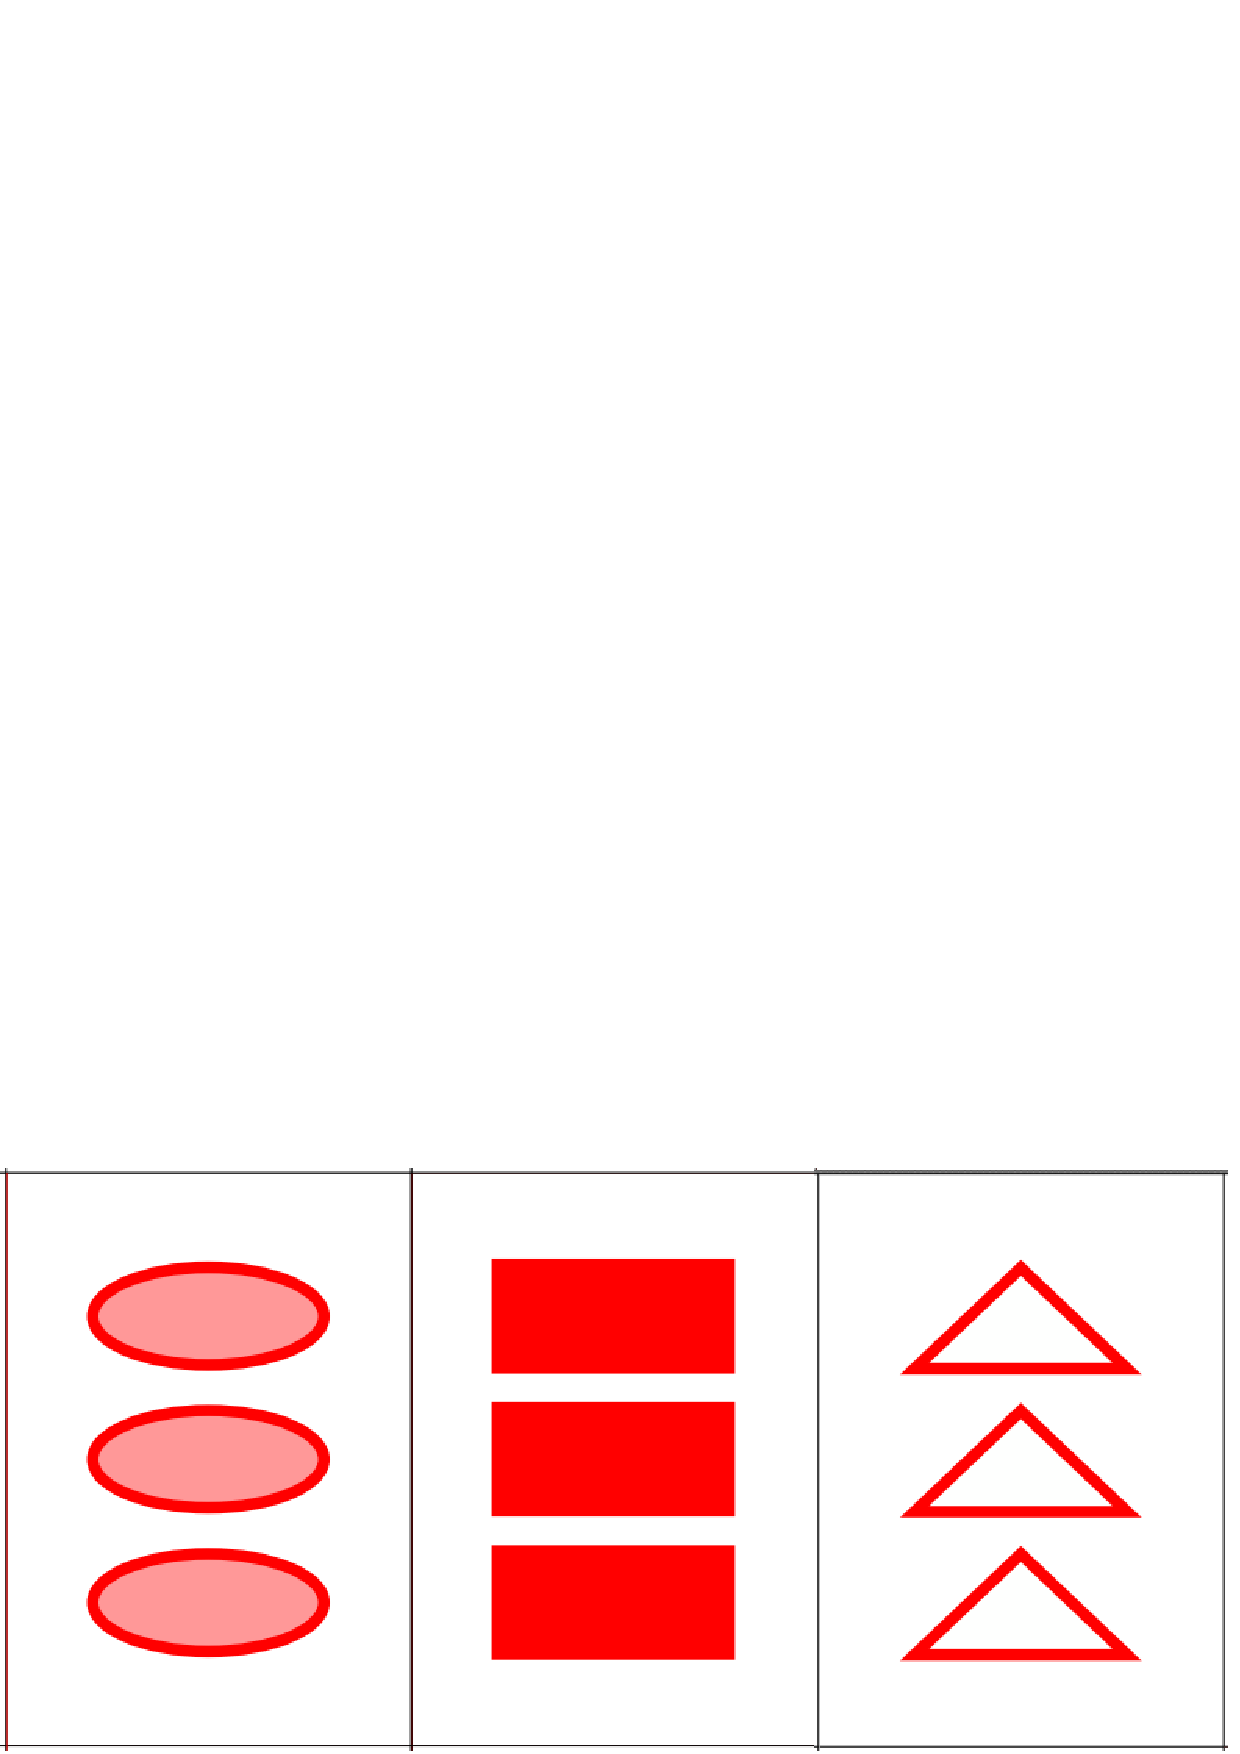
\includegraphics[width=0.8\textwidth]{obrazky/set_ano.png}\\
Táto trojica kartičiek tvorí SET: farba je rovnaká, tvar je na každej kartičke iný, podobne výplň a všetky majú rovnaký počet symbolov. \\
\\

\end{minipage}% This must go next to `\end{minipage}`
\hspace{20pt}\begin{minipage}{.4\textwidth}
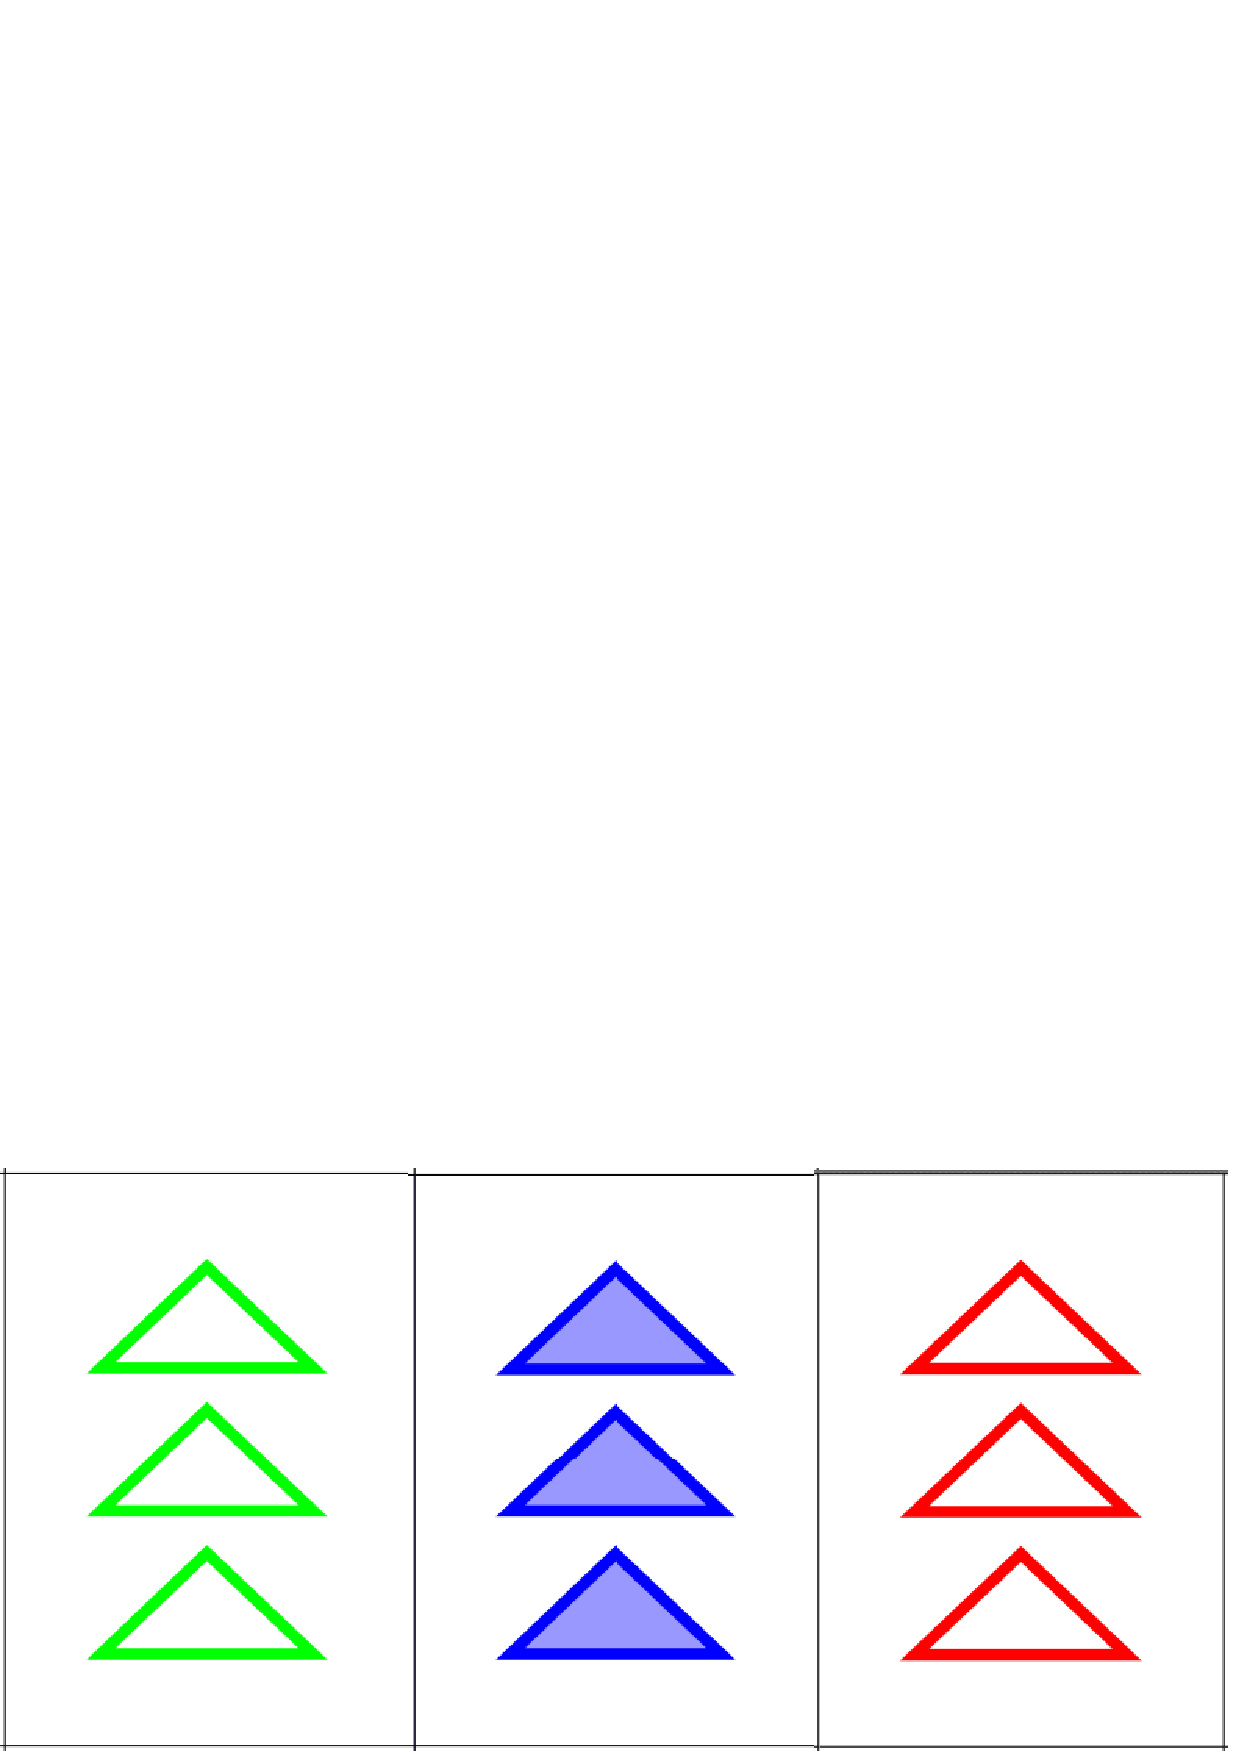
\includegraphics[width=0.8\textwidth]{obrazky/set_nie.png}\\
Táto trojica nie je SET. Síce majú všetky tri kartičky rovnaký počet symbolov, symboly sú rovnakého tvaru a každá kartička je inej farby, výplň na dvoch kartičkách je prázdna zatiaľ čo tretia je vyplnená polovične.
\end{minipage}

Po zamiešaní sa z~balíčka vyloží na stôl 12 kartičiek. Hráči medzi nimi hľadajú SETy. Ak sa to niekomu podarí, vykríkne \uv{SET!} a ukáže ho spoluhráčom. Ak je SET správny, hráč si ho vezme zo stola, namiesto neho sa vyložia nové tri kartičky a pokračuje sa v~hre. V~prípade, že sú hráči presvedčení, že sa medzi vyloženými kartičkami žiadny SET nenachádza, doložia na stôl ďalšie tri kartičky. Hra končí v~momente, kedy hráči vyčerpajú všetky kartičky. Cieľom hry je, samozrejme, pozbierať čo najviac SETov. Hra sa dá hrať v~takmer ľubovoľne veľkej skupine, z~praktických dôvodov sa najviac osvedčili trojice a štvorice.\\
\\
\kom Predtým, než sa pustíme do hrania, je vhodné so študentmi prejsť niekoľko trojíc kartičiek a pobaviť sa o~tom, ktoré trojice SETmi sú, ktoré nie a prečo, prípadne premietnuť rozloženie 12 kartičiek a hľadať v~nich SETy spoločne. \\
\\
Po zahraní niekoľkých kôl sa so študentmi pobavíme o~tom, akým spôsobom SETy hľadali, ktoré SETy sú na nájdenie jednoduchšie, prípadne iné ďalšie zaujímavosti, ktoré počas hry vypozorovali. K~tejto diskusii sa môžeme vrátiť neskôr v~priebehu seminára, keď sa budeme zaoberať kategorizovaním rôznych typov SETov.

\subsubsection*{Úlohy o~balíčku kariet}
\noindent \ul{27.2} Ak vyberiem dve ľubovoľné kartičky z~balíčka, koľko kartičiek existuje takých, aby s~pôvodnými dvoma tvorili SET a prečo? \end{tcolorbox}\ul{27.2} Ak vyberiem dve ľubovoľné kartičky z~balíčka, koľko kartičiek existuje takých, aby s~pôvodnými dvoma tvorili SET a prečo? \end{tcolorbox}

\rie Taká kartička je práve jedna, keďže charakteristiky prvých dvoch priamo určujú, aká variácia každej charakteristiky musí byť na poslednej kartičke (ak sa prvé dve kartičky v~charakteristike zhodujú, musí sa s~nimi zhodovať aj tretia, ak sú odlišné, aj tretia kartička sa musí odlišovať).\\
\\
\noindent \ul{27.3} Koľko rôznych SETov (kartičky sa v~rámci jednotlivých SETov môžu opakovať) sa nachádza v~celom balíčku?\end{tcolorbox}\ul{27.3} Koľko rôznych SETov (kartičky sa v~rámci jednotlivých SETov môžu opakovať) sa nachádza v~celom balíčku?\end{tcolorbox}

\rie  Na vytvorenie SETu potrebujeme tri kartičky. Prvú z~nich môžem bez akéhokoľvek obmedzenia vybrať spomedzi všetkých 81 kartičiek, druhá kartička sa dá vybrať 80 spôsobmi a z~predchádzajúceho vieme, že tretia kartička tvoriaca SET s~už dvoma zvolenými je práve jedna. Keďže však nezáleží na poradí, v~ktorom sme kartičky vyberali, vydelíme počet možností $81\cdot80$ počtom všetkých možných usporiadaní troch kartičiek, teda $6$. Celkom dostávame $\frac{81\cdot80}{6}=1080$ rozličných SETov.\\
\\
\noindent \ul{27.4} Z~balíčka vyberieme jednu kartičku. Koľkých rôznych SETov môže byť táto kartička súčasťou?\end{tcolorbox} \ul{27.4} Z~balíčka vyberieme jednu kartičku. Koľkých rôznych SETov môže byť táto kartička súčasťou?\end{tcolorbox} 
\rie  Z~predchádzajúceho plynie, že zvyšných 80 kartičiek v~balíčku vieme rozdeliť na 40 neprelínajúcich sa dvojíc, pričom každá táto dvojica bude tvoriť s~pôvodnou kartičkou SET.\\
\\
\kom Menej zdatným študentom môže s~pochopením vysvetlenia pomôcť vyložiť si na stôl konkrétne dvojice -- teda hľadať konkrétne SETy, ktorých je vybraná kartička súčasťou. \\
\\
\noindent \ul{27.5} Ako je možné ukázať, že v~danom rozložení kartičiek na stole sa nenachádza žiadny SET?\end{tcolorbox}\ul{27.5} Ako je možné ukázať, že v~danom rozložení kartičiek na stole sa nenachádza žiadny SET?\end{tcolorbox}
\rie  K~tomuto problému je možné pristupovať rôznymi spôsobmi, no všetky spája potreba skontrolovať všetky možné kombinácie a vylúčiť prítomnosť SETu. Zaujímavé je pozorovať, akú stratégiu študenti zvolia (v~porovnaní s~tým, ako postupovali pri hraní hry).  Nástavbou na túto úlohu môže byť otázka, ako dané rozloženie 12 kartičiek  skontrolovať čo najefektívnejšie.\\
\\

\noindent \ul{27.6} Je možné SETy nejako kategorizovať? Ako? Koľko SETov v~jednotlivých kategóriách je možné vytvoriť? Vieme správnosť našich výpočtov overiť pomocou nejakých predchádzajúcich úvah?\end{tcolorbox}\ul{27.6} Je možné SETy nejako kategorizovať? Ako? Koľko SETov v~jednotlivých kategóriách je možné vytvoriť? Vieme správnosť našich výpočtov overiť pomocou nejakých predchádzajúcich úvah?\end{tcolorbox}
\rie Táto úloha sa dá opäť uchopiť mnohými spôsobmi. Jedným z~nich môže byť roztriedenie SETov pomocou počtu charakteristík, ktoré majú kartičky spoločné. Každé rozdelenie, ktoré žiaci vymyslia, by ich však v~konečnom dôsledku malo priviesť k~rovnakému počtu SETov ako v~úlohe 2.\\
\\
\textbf{Záverečný komentár.} Hra SET je pre študentov (a nielen nich) veľmi atraktívna a majú tendencie sa odhodlane púšťať aj do predkladaných problémov. Stretnutie je tak príjemnou zmenou tempa a obsahu doterajšieho priebehu seminára

\subsubsection*{Doplňujúce zdroje a materiály}

Výborným sprievodcom plným zaujímavých úloh spolu s komentovanými študentskými riešeniami je možné nájsť na [TODO]. 


\newpage

\section*{Seminár 28}

\subsection*{Téma}
Matematická súťaž v~riešení úloh \textit{Náboj}\\
\\
\kom Druhé zo spomínaných stretnutí, ktoré je menej intenzívne v sprostredkovaní nových poznatkov, študentov preverí v tímovom riešení jednoduchších úloh. Príprava na seminár je rovnaká ako v Seminári 13, takže ak sme si s kolegami vytvorili dobrý vzťah počas prvého \textit{Náboja}, môžeme ich o spoluprácu poprosiť znova. Zároveň je vhodné študentov rozdeliť do iných družstiev než počas prvého náboja, aby si vyskúšali spoluprácu s ďalšími spolužiakmi. 

\section{Máj}

\section*{Seminár 30}

\subsection*{Téma}
Kvadratické rovnice

\subsection*{Ciele}
Precvičiť metódy používané pri práci s~kvadratickými rovnicami

\subsection*{Úlohy a riešenia}
\noindent \ul{30.1}  Určte všetky dvojice $a, b$ reálnych čísel, pre ktoré má každá z~kvadratických rovníc
$$ax^2 + 2bx + 1 = 0, \ \ \ \ bx^2 + 2ax + 1 = 0$$
dva rôzne reálne korene, pričom práve jeden z~nich je spoločný obom rovniciam.




\noindent \ul{30.2} 
Určte všetky dvojice $(a, b)$ reálnych čísel, pre ktoré majú rovnice
$$x^2 + (3a + b)x + 4a = 0, \ \ \ \  x^2 + (3b + a)x + 4b = 0$$
spoločný reálny koreň.




\noindent \ul{30.4} Reálne čísla $a$, $b$ majú túto vlastnosť: rovnica $x^2 -ax+b-1 = 0$ má v~množine reálnych čísel dva rôzne korene, ktorých rozdiel je kladným koreňom rovnice $x^2 - ax + b + 1 = 0$.

a) Dokážte nerovnosť $b > 3$.

b) Pomocou $b$ vyjadrite korene oboch rovníc.




\noindent \ul{30.5} Určte všetky hodnoty reálnych parametrov $p, q$, pre ktoré má každá z~rovníc
$$x(x - p) = 3 + q, \ \ \ \ x(x + p) = 3 - q$$
v~obore reálnych čísel dva rôzne korene, ktorých aritmetický priemer je jedným z~koreňov
zvyšnej rovnice.




\noindent \ul{30.6}  Pre ľubovoľné reálne čísla $k\neq \pm 1$, $p \neq 0$ a $q$ dokážte tvrdenie: Rovnica
$$x^2+ px + q = 0$$
má v~obore reálnych čísel dva korene, z~ktorých jeden je $k$-násobkom druhého, práve vtedy, keď platí $kp^2 = (k~+ 1)^2 q$.




\noindent \ul{30.7}   Na tabuli je zoznam čísel $1, 2, 3, 4, 5, 6$ a \uv{rovnica}
$$\frac{\fbox{$\phantom{7}$}}{\fbox{$\phantom{7}$}}x^2+\frac{\fbox{$\phantom{7}$}}{\fbox{$\phantom{7}$}}x + \frac{\fbox{$\phantom{7}$}}{\fbox{$\phantom{7}$}}= 0.$$
Marek s~Tomášom hrajú nasledujúcu hru. Najskôr Marek vyberie ľubovoľné číslo zo zoznamu, napíše ho do jedného z~prázdnych políčok v~\uv{rovnici} a číslo zo zoznamu zotrie. Potom Tomáš vyberie niektoré zo zvyšných čísel, napíše ho do iného prázdneho políčka a v~zozname ho zotrie. Nato Marek urobí to isté a nakoniec Tomáš doplní tri zvyšné čísla na tri zvyšné voľné políčka v~\uv{rovnici}. Marek vyhrá, ak vzniknutá kvadratická rovnica s~racionálnymi koeficientmi bude mať dva rôzne reálne korene, inak vyhrá Tomáš. Rozhodnite, ktorý z~hráčov môže vyhrať nezávisle na postupe druhého
hráča.




\section*{Seminár 31}

\section*{Seminár 32}

\section*{Seminár 33}

